\section{Overview}
\label{sec:arch_overview}

The Gateway Dashboard system follows a modern three tier architecture designed for clarity, scalability, and maintainability. The system separates concerns across three distinct layers: a user facing frontend built with Vue.js, a business logic layer implemented in NestJS, and a persistent data layer comprising MongoDB and Redis. This separation allows each layer to evolve independently while maintaining clear, well defined communication boundaries.

\subsection{Three-Tier Architecture}

Figure~\ref{fig:system_three_tier} illustrates the three tier architecture and the external services integrated into the system.

\begin{figure}[H]
\centering
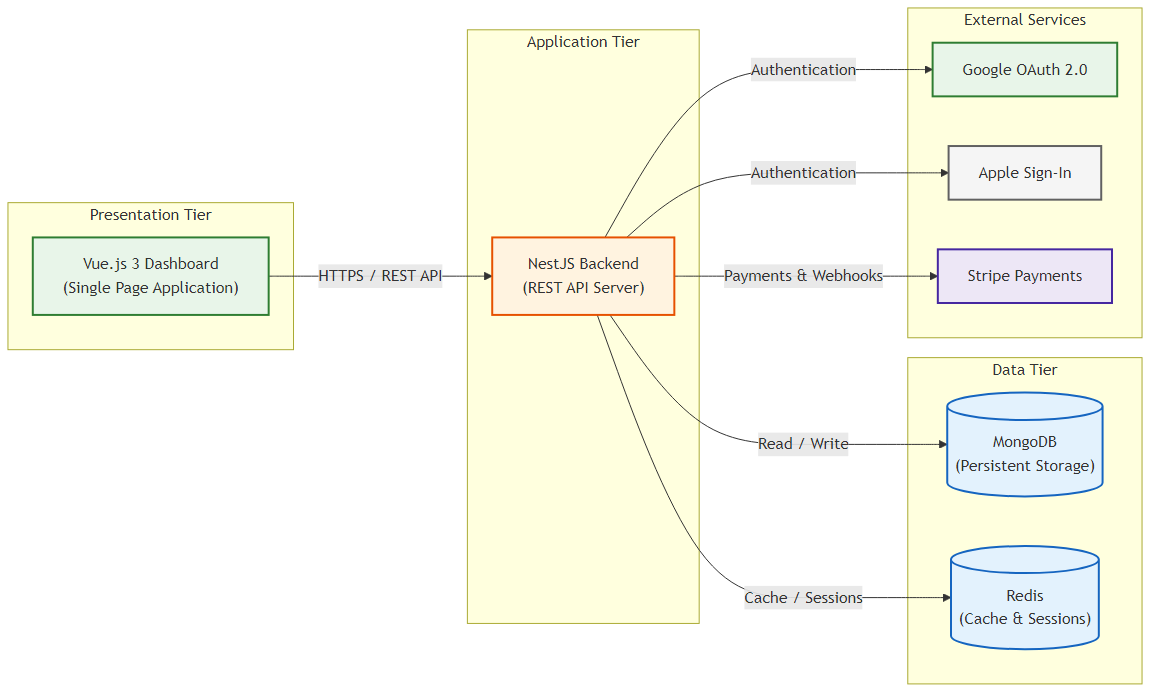
\includegraphics[width=0.85\textwidth]{images/system_three_tier.png}
\caption{Three-Tier System Architecture}
\label{fig:system_three_tier}
\end{figure}

The \textbf{Presentation Tier} is a Single Page Application built with Vue.js 3, running entirely in the user's browser. It communicates with the backend through standard HTTPS REST API calls. The \textbf{Application Tier} is a NestJS server that processes all business logic, including authentication, payment handling, and subscription management. The \textbf{Data Tier} uses MongoDB for persistent storage of user accounts, subscriptions, and plan definitions, alongside Redis for caching frequently accessed data and managing user sessions.

Three external services are integrated: \textbf{Google OAuth 2.0} and \textbf{Apple Sign-In} provide SSO authentication, while \textbf{Stripe} handles all payment processing and sends real time event notifications back to the backend via webhooks.

\subsection{Backend Module Organisation}

Figure~\ref{fig:backend_modules} shows how the backend is organised into distinct modules, each responsible for a specific area of functionality.

\begin{figure}[H]
\centering
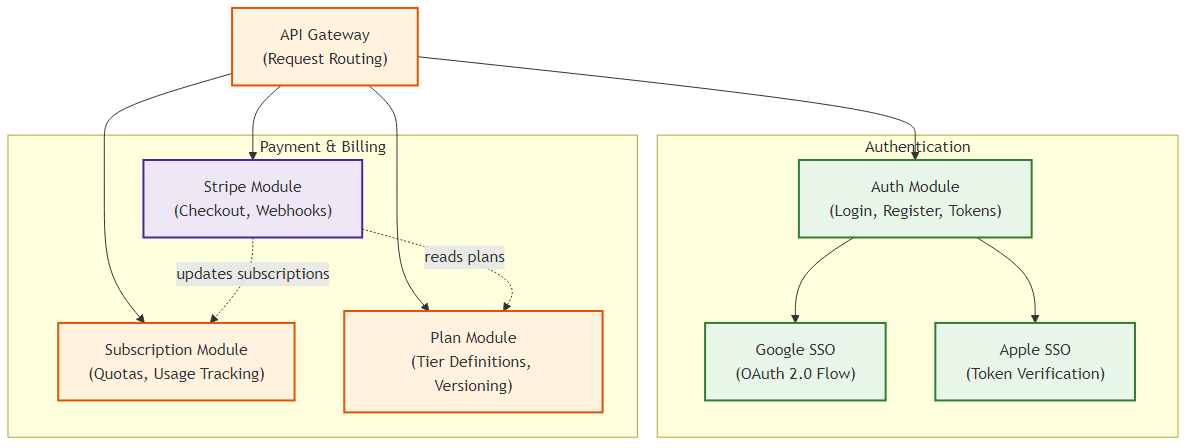
\includegraphics[width=0.75\textwidth]{images/backend_modules.png}
\caption{Backend Module Organisation}
\label{fig:backend_modules}
\end{figure}

The API Gateway routes incoming requests to the appropriate module. The \textbf{Authentication} group handles user login, registration, and token management, with dedicated submodules for Google SSO (using the OAuth 2.0 redirect flow) and Apple SSO (using token verification). The \textbf{Payment \& Billing} group consists of the Stripe Module (which manages checkout sessions and processes payment webhooks), the Subscription Module (which tracks each user's subscription status and usage quotas), and the Plan Module (which stores versioned plan definitions and caches them for performance). The dotted lines indicate cross module communication: the Stripe Module reads plan definitions when creating checkout sessions and updates subscription records when payment events occur.

\subsection{Communication Flow}

User interactions flow naturally through the system: when a user interacts with the frontend, the browser sends HTTP requests to the backend API, where incoming requests are validated and authorised. The backend then executes the required business logic, which may involve retrieving or storing data, checking cached values, or communicating with external payment and authentication services. Once processing is complete, the backend responds with the result, allowing the frontend to update the user interface accordingly.
